\chapter{\acl{PPG}}
\label{chap:PPG_teorie}

Fotopletysmografie (\acs{PPG}) je neinvazivní optická metoda sloužící k monitorování změn objemu krve v mikrovaskulárním řečišti tkáně, obvykle na prstu, zápěstí či ušním lalůčku \cite{Park2022}.
Zejména díky snadné integraci do nositelných zařízení (např. chytrých hodinek) a relativně nízkým nákladům na realizaci se \acs{PPG} stává klíčovým nástrojem pro dlouhodobé sledování kardiovaskulárních parametrů,
jako je tepová frekvence (HR), saturace krve kyslíkem (SpO\textsubscript{2}) či hodnocení variability tepových intervalů \cite{Orphanidou2018}.

Na obrázku \ref{fig:snimaniPPG} jsou schematicky znázorněny dvě základní měřicí konfigurace.
Transmisní režim (a) - zdroj světla a fotodetektor jsou na opačných stranách tkáně (typicky prst či ušní lalůček).
Reflexní režim (b) - zdroj i detektor leží na téže straně tkáně (např. zápěstí).

Metoda \acs{PPG} je založena na měření intenzity světla, která se po interakci s tkání dostane k detektoru.
Množství absorbovaného/odraženého světla závisí na aktuálním průtoku krve, který je modulován srdečními cykly \cite{Park2022}.

\begin{figure}[h]
	\centering
	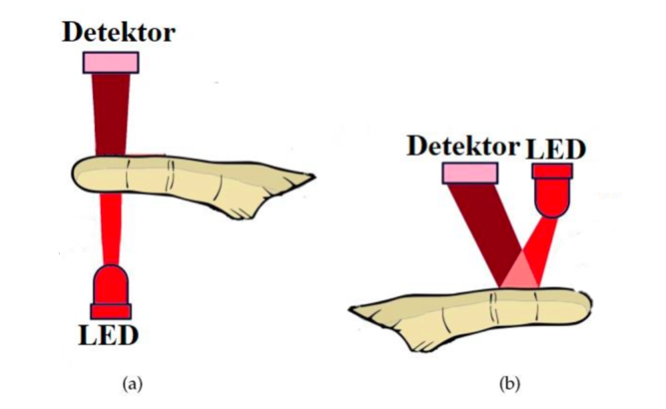
\includegraphics[width=0.8\textwidth]{./obrazky/snimaniPPG.png}
	\caption[Snímání PPG signálu]{Transmisní režim (a) a reflexní režim (b), upraveno z \cite{ENIKÖ}.}
	\label{fig:snimaniPPG}
\end{figure}

% ----------------------------------------------------------------------- %
\section{Složení \acs{PPG} signálu}

Jak ukazuje obrázek \ref{fig:signalPPG}, naměřený \acs{PPG} signál zahrnuje pulzní (AC) složku synchronizovanou se srdeční aktivitou a stabilní, nepulzní (DC) složku.
AC složka odráží periodické změny objemu arteriální krve v rozsahu typického frekvenčního pásma srdeční činnosti (zhruba 0,5--3~Hz) a je klíčová pro přesnou detekci \acs{TF}.
DC složka představuje základní linii danou absorpcí tkáně a žilní krve a ovlivňuje ji například barva kůže, okolní osvětlení a anatomické poměry měřené oblasti \cite{ENIKÖ, Park2022}.
Je důležité si uvědomit, že \acs{PPG} signál je inverzní k měřenému optickému signálu, protože reprezentuje objem krve v tkáni, nikoli množství světla odraženého zpět, což je patrné i z obrázku \ref{fig:signalPPG}.

Za počátek pulzu v \acs{PPG} signálu je obvykle označen nejnižší bod předcházející systolické fázi, který odpovídá bodu minimálního objemu krve v měřené oblasti.
Pro účel vypočítání \acs{TF} se využívá systolického vrcholu, což je bod s maximálním objemem krve.
Z více systolických vrcholů lze odvodit interval mezi srdečními údery a z toho stanovit \acs{TF}.
Po systolickém vrcholu přichází diastola, což je fáze srdečního cyklu, během které dochází k relaxaci srdečního svalu a plnění srdce krví.
V průběhu diastoly bývá často patrný typický dikrotický zářez, který odráží elastické vlastnosti cévní stěny a uzávěr aortální chlopně.
Jeho přítomnost a tvar mohou poskytovat užitečné informace o stavu krevního řečiště \cite{Orphanidou2018, Park2022}.

\begin{figure}[ht]
	\centering
	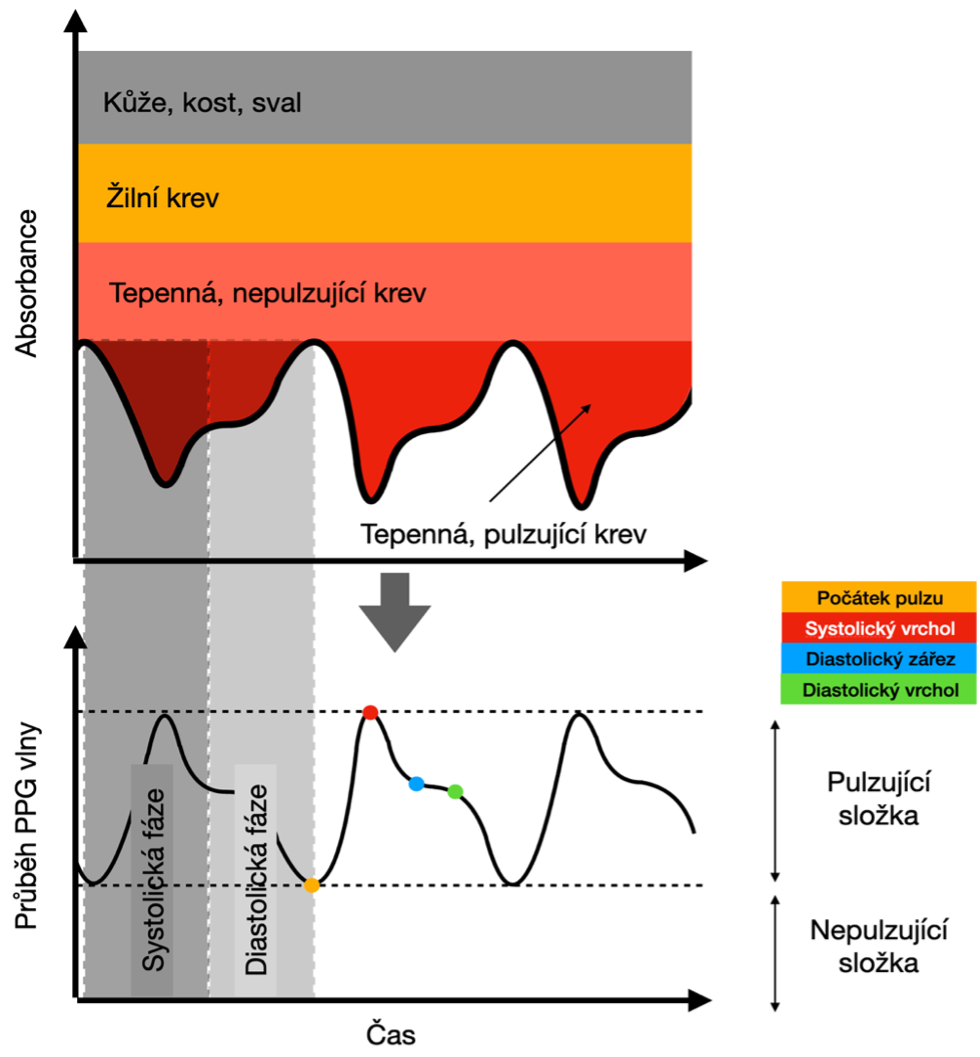
\includegraphics[width=0.8\textwidth]{./obrazky/signalPPG.png}
	\caption[Fiziologický popis PPG signálu]{Princip získání \acs{PPG} křivky a její popis, upraveno z \cite{Park2022}.}
	\label{fig:signalPPG}
\end{figure}